\documentclass[journal, a4paper]{IEEEtran}

\usepackage[utf8x]{inputenc}
\usepackage[english]{babel}

\usepackage{listings}

\usepackage{fancyvrb}
\usepackage{graphicx}
\usepackage{url}
\usepackage{amsmath}
\usepackage{tikz}
\usepackage{verbatim}

% Your document starts here!
\begin{document}

% Define document title and author
	\title{From centralized certification systems to more internet-like ones}
	\author{Alexandre Kervadec
	\thanks{Tutor : A.Guermouche}}
	\markboth{University of Bordeaux -- Master 2 Computing Sciences - Networking and mobile systems}{}
	\maketitle

% Write abstract here
\begin{abstract}
The current document is a study of a paper written by E.Gerck's paper : \textit{"Overview of Certification systems: X.509, CA, PGP and SKIP"}\cite{gerck1998overview}, but not only. First, it gives an overview of (the main) certification systems which are X.509 and CAs, PGP, SKIP, DANE and the Certificate transparency by Google, with thought on the pros and cons of each system, on a technical point of view and about the government's stranglehold on data exchanges.
\end{abstract}

% Each section begins with a \section{title} command
\section{Overview of certification systems}

X.509, CAs and PGP are the only technologies used to certify the authenticity of a user since the beginning of the 90's. But those technologies appear to have issues, for example, Google ''became aware of unauthorized digital certificates for several Google domains.''\footnote{https://googleonlinesecurity.blogspot.fr/2013/12/further-improving-digital-certificate.html} This kind of threat led some researchers to find new certification systems.

First sections show existing (sections \ref{x509} and \ref{pgp}) or extinguished (section \ref{skip}) certification systems. Then, further sections (\ref{dane} and \ref{certtrans}) introduce new, not implemented yet, technologies of digital certification which may solve current issues. 


\subsection{X.509 and CAs}
\label{x509}

X.509 and CAs\cite{rfc3647} infrastructure is based on a directory method.\\
With this kind of certification system, there are three different entities:

\begin{enumerate}
	\item \textbf{CA : Certification Authority}, an entity that controls authentication services and management of digital certificates. It can be public (like banks with their clients), commercial (such as \textit{Verisign} which sells its services) or private (like a company department, for an internal purposes).
	\item \textbf{Subscriber :} the entity which sends data to the CA to add it to his certificate. This entity is one that needs to be trusted by the \textit{user} entity.
	\item \textbf{User :} ask information about \textit{subscribers} to CA(s), it is central to the process, since the user party is relying on the informations given by \textit{CAs} and is thus at risk.
\end{enumerate}

The way that certification system works is the following:
\begin{itemize}
	\item A subscriber gives informations to the CA, in order to create a digital certificate for itself in the CA directory.
	\item The CA receives the information and puts it in a certificate.
	\item A user (the public in general) receives a certificate from a subscriber. In order to authenticate this subscriber, the client asks to the CA if the transmitted certificate matches with the subscriber's identity.
	\item The CA answers to the user to give him the precious informations about the subscriber's identity.
\end{itemize}

Let us get an example: \textit{user1} wants to prove his identity to \textit{Bob} with a CA (Jack) (Figure 1).\\
First, Oscar needs to get a certificate signed by Jack, so he requests it from Jack with some informations about himself. Jack makes the certificate and signs it, then he sends it back to Oscar.\\
Now Bob wants to communicate with Oscar, so to prove his identity, Oscar gives to Bob his certificate (forged by Jack). In order to verify Oscar's identity, Bob asks to Jack if the certificate is valid. Then Jack examines this certificate and answers to Bob, the answer can be:
\begin{itemize}
	\item Yes, it is valid
	\item No, it is not valid
	\item Not sure about its validity
\end{itemize}
With that information, Bob can choose to trust or not Oscar.

\begin{figure}[!h]
	\begin{center}
		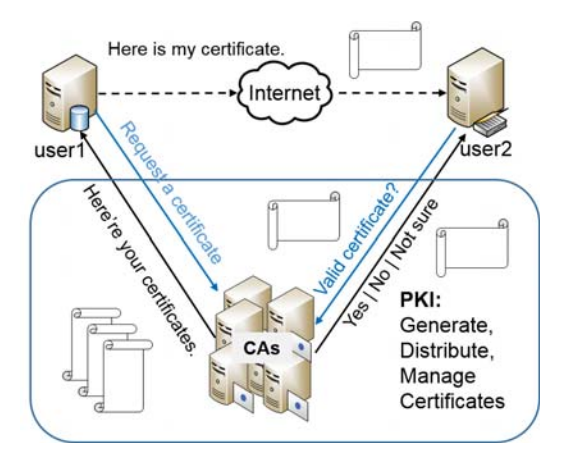
\includegraphics[scale=0.45]{pki.png}
		\caption{Diagram of the X.509 and CAs process (from \cite{wang2015domain})}
		\label{fig:pki}
	\end{center}
\end{figure}

There is a not outwardly perceived entity in this system, it is the Naming Authority (DN). It provides to the CA a unique distinguished name (DN) which matches with the subscriber's identity in the certificate.\\
Note that the CA can double in NA, but they provide two different services: the CA certificate refers to a name but does not denote it, the NA does.\\

The main concerns about authentification services provided by CAs are :

\begin{itemize}
	\item The content of a certificate needs to be discussed, as well as certificate revocation. For example, a subscriber can generate multiple DN for a same CA or the same DN to multiple CAs, so maybe, a better subscriber identificator needs to be added.
	\item Are the validation procedures for the certified data that is included in a certificate solid enough? Because each CA has its own self-defined rules (Certification Practice Statement\footnote{CPS}), which can be completly different from one CA to another.
\end{itemize}

There is a big problem with CPS (Certification Practice Statements), that can be noted such as flexibility (for pros), because each CA answer has specific needs, so that is a sort of lack of harmonization.

Also, regarding the law, CAs deny any leak of information from themselves \cite{gerck1998overview}.

Some kind of conclusion about harmonization (lack of), in a world wide vision, if space there is.

\subsection{PGP (Pretty Good Privacy)}
\label{pgp}

PGP, created thanks to Phil Zimmermann research. It has two parts: certification and encryption, the following text only deals with certification.\\
Compared to X.509, PGP is more \textit{internet-like}, this because of its \textit{introducer-model} base.\\
PGP depends on a chain of authenticators: the users themselves. This chain forms a ring, but not in a closed way but in a mathematical way like a list or a \textit{web-of-trust}. You may not knows everyone in this ring, but you can assume that you will know somebody who know this user. You can also assume that different rings can have some contact points to guarantee the referrals.

Thus, we can figure out that PGP breaks the traditional hierarchical trust architecture with this \textit{web-of-trust} approach.\\

\begin{figure}[!hbt]
	\begin{center}
		
		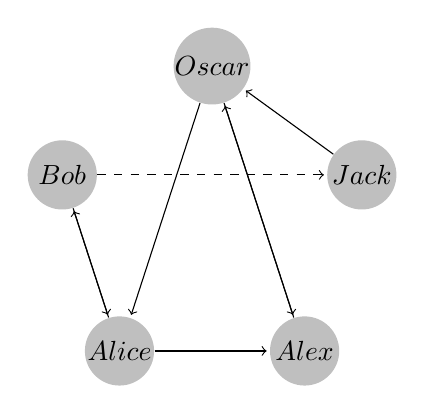
\begin{tikzpicture}[shorten >=1pt,->]
			\tikzstyle{vertex}=[circle,fill=black!25,minimum size=25pt,inner sep=0pt]

			\foreach \name/\angle/\text in {P-1/234/Alice, P-2/162/Bob, 
                                  P-3/90/Oscar, P-4/18/Jack, P-5/-54/Alex}
				\node[vertex,xshift=6cm,yshift=.5cm] (\name) at (\angle:2cm) {$\text$};
    
			\draw (P-1) -- (P-5);
			\draw[dashed,->] (P-2) -- (P-4);
			\draw (P-4) -- (P-3);
			\draw (P-3) -- (P-1);
			\draw (P-1) -- (P-2);
			\draw (P-2) -- (P-1);
			\draw (P-3) -- (P-5);
			\draw (P-5) -- (P-3);
  
		\end{tikzpicture}
		\caption{Communities of trust: Jack introduces Oscar to Bob's public-key certificate before Bob receives it.}
		\label{fig:web-of-trust}
	\end{center}
\end{figure}

Let us get an example\footnote{Example from ''The PGP trust model''\cite{caronni2000}} (Figure \ref{fig:web-of-trust}): Bob wants to exchange data with Oscar, whom he didn't know before. But Jack, a colleague of Bob's, signs Oscar's public-key certificate which he knows is authentic.\\
Oscar then forwards his signed certificate to Bob who wishes to communicate with Oscar privately.\\
Bob, who knows and trusts Jack as an \textit{introducer}, finds out, after verification, that Jack is among Oscar's certificate signer. Therefore, Bob can be confident that Oscar's public key is authentic.

However, had Bob not known or trusted Oscar's signers, including Jack, he would have been skeptical about the authenticity of Oscar's public-key. Oscar would then have to find another introducer whom Bob trusts to sign Oscar's public-key certificate. This is illustrated in Figure \ref{fig:web-of-trust}.\\
The dotted arrow indicates ''Bob trusts Jack as introducer'' and the solid arrow indicates ''Jack trusts Oscar’s public key validity''. 


PGP also includes a public-key certificate and an introducer trustwhorthiness. They have different levels, for a public-key certificate they are:
\begin{itemize}
	\item \textit{Undefined:} we cannot say wether this public-key is valid or not.
	\item \textit{Marginal:} this public-key \textit{may} be valid but we cannot be sure.
	\item \textit{Complete:} we can be fully confident that this public-key is valid.
\end{itemize}
For an introducer, those levels of trustworthiness are the following:
\begin{itemize}
	\item \textit{Full:} this public-key is fully trusted to introduce another public-key.
	\item \textit{Marginal:} this public-key can be trusted to introduce another public-key, but, it is uncertain whether it is fully competent to do that.
	\item \textit{Untrustworthy:} this public-key should not be trustedto introduce another, therefore any occurence of this key as a signature on another public-key should be ignored.
\end{itemize}

Only the trustworthiness of public-key's validity is automatically evaluated by PGP. The introducer's worthiness is manually assigned by each user of to the public key, and exists only within each individual user's public-key ring\footnote{PGP allows users to have files representing multipke \textit{key rings} to store public or secret keys\cite{caronni2000}.}.

The big point is the use of such a tool in a world wide range: that is reasonably not possible. We can assume it can be used in a little group, where trustworthiness is effective, but in a wider area, it is problematic to trust such a number of people, or find trusted introducers. Furthermore, in a commercial use, there is no entity responsible when something goes wrong.


\subsection{SKIP (Simple Key-Management for Internet Protocol)}
\label{skip}

SKIP implements a linked-chain of two-sided node authenticators, where each node derives its informations from a sort of \textit{directory service}.\\
The problem is that SKIP happens at a low level, so it is transparent to the user; also assuming that the user has no control over security or other certification choices. So it has to be complemented by a second higher level protocol. Furthermore, SKIP does not support IP translation (such as NAT behind a firewall), that makes it quite useless.\\
So that protocol imediatly looks inappropriate for our study. In an other way, SKIP does not exist anymore, so it is pointless to go further in its study.


\subsection{Thoughts about X.509, CAs and PGP}
\label{thoughts_old}

To be used in a commercial way, X.509, CAs and PGP need a centralized certification control system (a matter of responsibility).
However, there is a struggle between this need of centralization and the decentralized internet architecture.
It shows us the futility of certification authority for the whole world, since we have no centralized world governance or law.\\
The main question is:\\
\textit{How can we have a main control over an internet environment, to assure the security of the data and legitimacy of users/servers?}\\
Some answers have been provided since then (thus since the publication of the original article).


\subsection{DANE (DNS-Based Authentication of Named Entities)}
\label{dane}

DANE is not implemented yet, but an IETF team is working on the standard.\\
It has begun with a simple assertion: why use a new trust infrastructure if we already have to use DNS to resolve a domain name?\\
From here, DNS must be securised, knowing that it is easily to set a MITM with DNS cache poisoning \cite{aa04} using the Kaminsky attack \cite{bor08}. That is the main purpose of DNSSEC: secure DNS. DANE allows to store keys in DNS. Thereby, \verb$www.example.org$ would be able to secure \verb$https://www.example.org$ without using a suspicious third part, just by putting its keys in the domain name that it controls. By its arborescent nature, \verb$example.org$ shall not be able to cheat on \verb$example.com$.\\

Lets give us an example:\\
From the classic schem, we have \textit{Alice}, the subscriber (\verb$alice.example.com$), \textit{Bob} its client, and \textit{Charlie}, the serious AC. There are three different scenarios:
\begin{itemize}
	\item \textit{Type 0:} Alice has got a certificate delivered by Charlie and is really satisfied by it. But Alice is afraid that \textit{Oscar} (a bad AC) might forge a false certificate for his website. So Alice uses DANE to tell in DNS that Charlie and only Charlie is its AC.
	\item \textit{Type 1:} Alice has got a certificate delivered by Charlie, but fears that Charlie might give its certificate to bad people. So Alice uses DANE to publish in DNS the origin of its certificate.
	\item \textit{Type 2:} that is the \textit{max scenario} in DANE. Alice doesn't trust ACs anymore, so it decides to emit it via DANE on DNS, that gives the entire responsibility on DNS servers. 
\end{itemize}

This type is in a new register called TLSA\footnote{TLSA doesn't stand for anything: it is just the name of the RRtype (Record Resource type).} in DNS. Her is an example of a TLSA register:\\
\begin{Verbatim}[fontsize=\small]
_443._tcp.www.example.com. IN TLSA (
	0 0 1 d2abde240d7cd3ee6b4b28c54df0&34b9
	7983a1d16e8a410e4561cb106618e971 )
\end{Verbatim}
With:
\begin{itemize}
	\item \verb$443$ : the port used.
	\item \verb$tcp$ : the protocole used.
	\item \verb$www.example.com$ the domain name.
	\item \verb$0 x x$ : the type used, here it is a type 0 (\verb$1 x x$ for type 1 and \verb$2 x x$ for type 2).
	\item The rest is the certificate itself.
\end{itemize}

\begin{figure}[!hbt]
	\begin{center}
	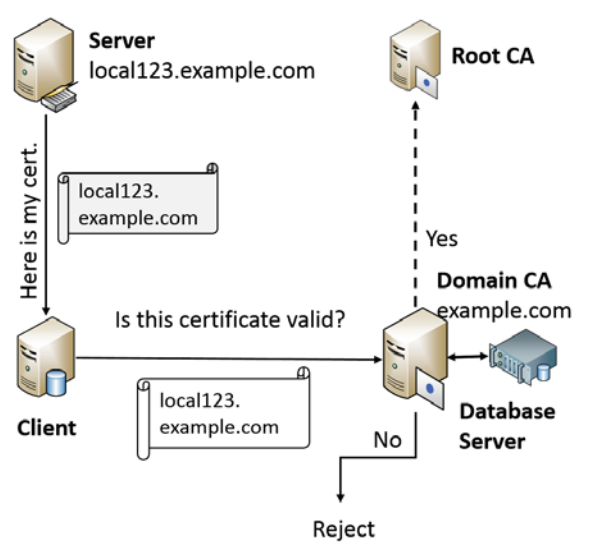
\includegraphics[scale=0.4]{danereq.png}
	\label{fig:pki}
	\caption{Process of certificate verification (from \cite{wang2015domain})}
	\end{center}
\end{figure}

As we said before, DNS is not secured, so DNSEC has been deployed. DNSSEC is a protocol that allows to the DNS server (master) to encrypt and sign its answer with a public key cryptographic system. It also permits to return a \verb$NXDOMAIN$ type (''No Such Domain'').\\
Nervertheless DNSSEC has some vulnaribilities such as:
\begin{itemize}
	\item Replay attacks
	\item Attacks against intermediaries: because of the hierarchic and centralized approach of DNS (there is only one root), the responsibility of intermediaries is really high and a remote control by a thief should be damaging (the thief controls the domain thus). History has proved that some of those intermediaries are not that trustworthy \cite{dan08} \cite{utk11}.
\end{itemize}

To make a conclusion about DANE, we have multiple points to point out:
\begin{itemize}
	\item Introducing a new register TLSA shall be very complicated, knowing that things are not moving that fast in DNS\footnote{Like it use to be with EDNS introduction few years ago.}.
	\item The end to end validation necessity end to end is quite disturbing knowing that there is no standard and deployable solution for wide use  about the last kilometer securisation.
	\item DNSSEC is not possible behind a DNS proxy (which filters/breaks DNS answers to the point of creating a DoS for all TLS services.
\end{itemize}

Therefore, DANE is on a good way, particularly for communications between servers, where there is no (not many) constraints of security are (more) easily achievable. 

\subsection{Sovereign keys}
\label{sovkeys}

Sovereign keys are an Electric Frontier Foundation (EFF\footnote{www.eff.org}) proposition.

A sovereign key is a cryptographic pair of keys where the public key is associated to a domain name (or a subdomain) to create a trust anchor\footnote{A trust anchor is an authoritative entity for which trust is assumed and not derived \cite{wallace2010}.} for itself.\\
This association \textit{public key/domain name} is registered in a append-only data structure, kept on servers named ''\textit{timeline servers}''. There is a small number, around 10-20, of these \cite{eck2014}.\\
The private part of the sovereign key (private key) allows to sign certificates of which the CN is the domain (or subdomain) name which it is associated to.\\
During a handshake with a TLS server, the certificate is sent with its protected domain key signature, by the same mechanism than as a TLS transaction based on PKIX. The client has then the possibility to recover the public key associated with that sovereign key from the timeline servers to check the key's validity, that the domain is the same as the one in the current transaction and that it signs the receive certificate.

A sovereign key has a cycle of life that begins with the generation of a cryptographic pair of keys	by the domain administrator (who wants to use TLS server on his domain). This administrator must at first, prove that he really is controlling his domain before seeing it in public data-structures.\\
To do so, he must give his certificate (of which the CN covers his domain name declared protected by the sovereign key) signed by an AC recognized by the \textit{timeline servers}\footnote{The list of AC's recognized by the timeline servers is public and must be up to date, by conception.} or through DANE (once the standard has been published and implemented).\\
During the public key registering by the timeline servers, proofs of control on the domain are examined and added to the sovereign key metadata. Other data are added such as:
\begin{itemize}
	\item Expiration date.
	\item Names (and ports) of TLS services uses and protected by the sovereign key.
	\item A list (that may be empty) of domain names whose sovereign keys are granted to revoke (in case of loss of control of the private part of the sovereign key) the entry being entered.
\end{itemize}
A data-structure of sovereign keys being a append-only list, once the sovereign key is entered, it cannot be removed. The domain administrator can only modify informations by pushing data in that data-structure. To remove a sovereign key (in the case the private key has been lost), the domain adminstrator needs to use a domain name with a sovereign key granted to modify its own sovereign key (thus present in the list of his own sovereign keys, see in the item list below) or wait for his sovereign key's expiration date. 

This structure is useful because it protects from DNS or AC compromise of sovereign key by smurf attacks\footnote{Attacker able to give proof of domain control.}. It also needs to be used with care, because an unadvised administrator may lose control of its own domain.\\

The drawbacks of this systems are:
\begin{itemize}
	\item A service declared protected in a data-structure of a timeline server needs to use a secure protocol (HTTPS instead of HTTP for example) to avoid downgrade attacks. It may be seen as an intrusion into the freedom of a service governance.
	\item Loosing a private key may result in a long term denial of service if no domain sovereign key is granted to modify the private key's sovereign key.
	\item A compromized private key may lead to a total loss of control of the entire domain.
	\item The use of ACs to certify the domain owner is the big flaw of this system.
\end{itemize}

\subsection{CATA: Certificate Authority Transparency and Auditability}
\label{certtrans}

This protocol has been developed by a Google team a few years ago \cite{LL11}. It is still under development \cite{certtransp2013} so it is not implemented and deployed yet. It also has to be improve, like everything in computing science, in the early years.\\
CATA's purpose is a public list of all certificates that are emitted by CAs. Thus, clients are allowed to search in that public list, and verify that the received certificate is in that list, to be validated (if it is not in the list, it shall be rejected).\\
In that way, a(conscientious) domain administrator can have access to that list and monitor all fraudulent certificates for his domain.\\
For the moment, there are plenty of questions to answer like :
\begin{itemize}
	\item Who should hold those lists?
	\item How many lists should be created?
	\item How should the revokation work?
	\item What should happen if a certificate is no longer available (path unreachable)?
\end{itemize}


\section{Conclusion}
\label{conclusion}

Despite the great need to replace the PKIX security model\footnote{X.509 and CAs}, none of those presented above may be valid, or well tested to be implemented on a large scale (world wide).

Therefore, the best model may be the sovereign keys system associated with the DANE control of a domain control certification, as soon as security problems are fixed in DANE with DNSSEC.\\

Otherwise, another point of view that needs to be discussed, is the economic impact of such a revolution: companies like VeriSign\footnote{www.verisign.com} or GeoTrust\footnote{www.geotrust.com} may face bankruptcy with the removal of all CAs. Knowing that they are big deciders in the internet activity, they detain a great lever on governments (because money leads capitalism), to stop or at least slow down the deployment process of a new certification system.

In general, to fit the Internet, experience has shown that we need to develop systems that are the most distributed possible, like the internet paradigm.

\pagebreak

\nocite{*}

\begin{thebibliography}{99}

\bibitem{gerck1998overview} E.Gerck, Overview of Certification Systems: X. 509, CA, PGP and SKIP, 1998.

\bibitem{skip1995} Ashar Aziz, Tom Markson, Hemma Prafullchandra, Sun Microsystems, Inc., v.06, 1995. https://tools.ietf.org/html/draft-ietf-ipsec-skip-06

\bibitem{skip2010user} Oracle, SunScreen SKIP User's Guide, Release 1.1, 2010. %http://docs.oracle.com/cd/E19957-01/805-5743/6j5dvnrfs/index.html

\bibitem{caronni2000} Caronni, G. (2000). Walking the web of trust. In Enabling Technologies: Infrastructure for Collaborative Enterprises, 2000.(WET ICE 2000). Proeedings. IEEE 9th International Workshops on (pp. 153-158). IEEE. %http://system.khl.mydns.jp/college/WOT/The_PGP_Trust_Model.pdf

\bibitem{bor08} Stéphane Bortzmeyer. Comment fonctionne la faille kaminsky ? http://www.bortzmeyer.org/comment-fonctionne-la-faille-kaminsky.html, 2008.

\bibitem{aa04} D. Atkins and R. Austein. Rfc 3833 : Threat analysis of the domain name system (dns). http://www.
ietf.org/rfc/rfc3833.txt, 2004.

\bibitem{dane2012} P Hoffman, J Schlyter, The DNS-based authentication of named entities (DANE) transport layer security (TLS) protocol: TLSA, 2012. https://www.rfc-editor.org/rfc/pdfrfc/rfc6698.txt.pdf

\bibitem{LL11} Ben Laurie and Adam Langley. Certificate authority transparency and auditability. http://www.links.
org/files/CertificateAuthorityTransparencyandAuditability.pdf, 2011.

\bibitem{certtransp2013} Laurie, B., Langley, A., \& Kasper, E. (2013). Certificate transparency (No. RFC 6962). %https://www.rfc-editor.org/rfc/pdfrfc/rfc6962.txt.pdf

\bibitem{rfc3647} Solo, D., Housley, R., \& Ford, W. (1999). Internet X. 509 public key infrastructure certificate and CRL profile. %http://tools.ietf.org/html/rfc2459

\bibitem{dan08} Dancho Danchev. Hackers hijack dns records of high profile new zealand sites. http://m.zdnet.com/blog/security/hackers-hijack-dns-records-of-high-profile-new-zealand-sites/3185, 2008.

\bibitem{utk11} Utkarsh. Domaining.com hacked. http://dotsutra.com/domain-names/industry-news/domaining-com-hacked/, 2011.

\bibitem{wallace2010} Wallace, C. Trust Anchor Format. No. RFC 5914. 2010.

\bibitem{eck2014} P. Eckersley, ''Sovereign key cryptography for internet domains'', online, 2012, https://git.eff.org/?p=sovereign-keys.git;a=blob\_plain;f=sovereign-key-design.txt;hb=master, last retrieved on December 21, 2014.

\bibitem{wang2015domain} Wang, Xinli, Yan Bai, and Lihui Hu. "Domain based certification and revocation." Proceedings of the 2015 International Conference on Security and Management, SAM. Vol. 15. 2015.

\bibitem{mf2011} Maury, Florian. "La fin annoncée des autorités de certification? Alternatives: TOFU, Convergence, CATA, Clés souveraines, DANE." Convergence 10 (2011): 509.

\bibitem{correia2015dns} Correia, Miguel Medeiros, and Mustafa Tok. DNS-based Authentication of Named Entities (DANE). Technical report, Universidade do Porto, 2011–2012, 2015.

\end{thebibliography}

% Your document ends here!
\end{document}
